\documentclass[11pt,a4paper]{article}

\usepackage[T1]{fontenc}
\usepackage[utf8]{inputenc}
\usepackage{lmodern}
\usepackage[margin=2.3cm]{geometry}
\usepackage{amsmath}
\usepackage{booktabs}
\usepackage{array}
\usepackage{xcolor}
\usepackage{listings}
\usepackage{float}
\usepackage{tikz}
\usetikzlibrary{arrows.meta,positioning,automata}
\usepackage[hidelinks]{hyperref}

\lstset{basicstyle=\ttfamily\footnotesize, columns=fullflexible, keepspaces=true, frame=single,
        framesep=3pt, xleftmargin=4pt, xrightmargin=4pt, showstringspaces=false}

\newcommand{\First}{\textsc{First}}
\newcommand{\Follow}{\textsc{Follow}}
\newcommand{\Closure}{\textsc{Closure}}
\newcommand{\Goto}{\textsc{Goto}}
\newcommand{\Action}{\textsc{Action}}
\newcommand{\code}[1]{\texttt{#1}}
\newcommand{\todo}[1]{\noindent\fbox{\parbox{\dimexpr\linewidth-2\fboxsep-2\fboxrule}{\textbf{TODO (group):} #1}}}

\title{Formal Languages Project\\[4pt]
\large FIRST/FOLLOW, LL(1) and SLR(1) parsers, and evaluation of an SDD}
\author{Simon Alejandro Vasquez Medina \and Miguelangel Calderon Figueredo \and Sebastian Urrego Ramirez}
\date{November 2026}

\begin{document}
\maketitle

\section{Introduction}

This report describes our implementation of the project. It covers three items:
\begin{itemize}
  \item \textbf{Item~1:} the \First{} and \Follow{} sets of a context-free grammar.
  \item \textbf{Item~2:} the table-driven LL(1) parser and the SLR(1) parser.
  \item \textbf{Item~3:} the evaluation of a syntax-directed definition (SDD) on the parse tree of a string, with the dependency-graph method.
\end{itemize}
Everything is written in Python~3 using only the standard library. Every algorithm follows the book
\emph{Compilers: Principles, Techniques, and Tools} (Aho, Lam, Sethi, Ullman, 2nd edition). The
\code{README.md} file explains how to run each part.

\section{Book sections, algorithms and data structures}

Table~\ref{tab:map} shows, for each part of the program, which part of the book it follows.

\begin{table}[H]
\centering
\small
\begin{tabular}{@{}lll@{}}
\toprule
File / function & What it does & Book \\
\midrule
\code{first\_follow.py}: \code{compute\_first} & $\First(X)$ for every symbol & Sec.~4.4.2 \\
\code{first\_follow.py}: \code{first\_of\_string} & $\First(X_1X_2\cdots X_n)$ & Sec.~4.4.2 \\
\code{first\_follow.py}: \code{compute\_follow} & $\Follow(A)$ for every nonterminal & Sec.~4.4.2 \\
\code{ll1.py}: \code{is\_ll1} & Test of the LL(1) condition & Sec.~4.4.3 (start) \\
\code{ll1.py}: \code{build\_ll1\_table} & Predictive parsing table $M$ & Algorithm 4.31 \\
\code{ll1.py}: \code{ll1\_parse} & Table-driven predictive parser & Algorithm 4.34, Fig.~4.20 \\
\code{slr1.py}: \code{augment} & Augmented grammar ($S' \to S$) & Sec.~4.6.2 \\
\code{slr1.py}: \code{closure} & $\Closure(I)$ & Fig.~4.32 \\
\code{slr1.py}: \code{goto} & $\Goto(I, X)$ & Sec.~4.6.2 \\
\code{slr1.py}: \code{canonical\_collection} & Canonical collection of LR(0) items & Fig.~4.33 \\
\code{slr1.py}: \code{build\_slr\_table} & \Action{} and \Goto{} tables, conflicts & Algorithm 4.46, Sec.~4.5.4 \\
\code{slr1.py}: \code{slr1\_parse} & LR-parsing algorithm & Algorithm 4.44, Fig.~4.36 \\
\code{sdd\_rules.py} & The SDD, in the format of Fig.~5.1 & Sec.~5.1.1 \\
\code{sdd.py}: \code{build\_graph} & Dependency graph & Sec.~5.2.1 \\
\code{sdd.py}: \code{topological\_order} & Topological sort, cycle detection & Sec.~5.2.2 \\
\bottomrule
\end{tabular}
\caption{Correspondence between the program and the book.}
\label{tab:map}
\end{table}

\paragraph{Data structures.}
\begin{itemize}
  \item \textbf{Grammar.} A \code{Grammar} object stores:
  \begin{itemize}
    \item the list of nonterminals;
    \item the list of terminals, sorted in ASCII order;
    \item the productions, as a list of pairs \code{(head, body)}, where \code{body} is a list of symbols and $\varepsilon$ is the empty list.
  \end{itemize}
  A production is identified by its position in that list.
  \item \textbf{FIRST and FOLLOW.} Dictionaries from each symbol to a Python \code{set}. The letter \code{e} stands for $\varepsilon$ and \code{\$} is the end marker. Both are computed by applying the rules of Section~4.4.2 repeatedly until no set changes.
  \item \textbf{LL(1) table.} A dictionary \code{table[(A, a)] = production number}. A missing entry is an error entry.
  \item \textbf{LL(1) parser.} The stack (a Python list) holds parse-tree nodes. Each node is an object with \code{symbol}, \code{production}, \code{children} and \code{attrs}.
  \item \textbf{LR(0) items.} An item is a pair \code{(production number, dot position)}, and a set of items is a Python \code{set}. The canonical collection is a list of sets, where the index is the state number. The \Goto{} function of the automaton is a dictionary \code{transitions[(i, X)] = j}.
  \item \textbf{SLR table.} \Action{} is a dictionary \code{action[(i, a)]} whose value is \code{("shift", j)}, \code{("reduce", k)} or \code{("accept",)}. \Goto{} is a dictionary \code{goto\_table[(i, A)] = j}.
  \item \textbf{SDD.} A dictionary from each production to its list of rules. A rule is a tuple \code{(defined attribute, used attributes, function)}.
  \item \textbf{Dependency graph.} A vertex is the pair \code{(node, attribute name)}. Its edges are stored as adjacency lists: \code{edges[v]} is the list of vertices that depend on~$v$.
\end{itemize}

\section{Items 1 and 2}

\subsection{Our grammar}

As the grammar of our own we use nested lists, such as \code{[x;[x;x];[]]}:
\begin{center}
\begin{tabular}{l}
\code{3}\\
\code{S -> [L] x}\\
\code{L -> SR e}\\
\code{R -> ;SR e}
\end{tabular}
\qquad\qquad
\begin{tabular}{rl}
(1) & $S \to [\,L\,]$\\
(2) & $S \to x$\\
(3) & $L \to S\,R$\\
(4) & $L \to \varepsilon$\\
(5) & $R \to\ ;\,S\,R$\\
(6) & $R \to \varepsilon$
\end{tabular}
\end{center}
The productions are numbered as in Fig.~4.37 of the book. Number~0 is the augmented production $S' \to S$.

\subsection{FIRST and FOLLOW}

Output of \code{python main.py --sets < tests/report\_grammar\_strings.txt}:
\begin{lstlisting}
First(L) = {[, x, e}
First(R) = {;, e}
First(S) = {[, x}
Follow(L) = {]}
Follow(R) = {]}
Follow(S) = {;, ], $}
\end{lstlisting}

\subsection{LL(1) test and LL(1) table}

The function \code{is\_ll1} checks the condition at the beginning of Section~4.4.3 for every pair of
productions $A \to \alpha \mid \beta$. The first two conditions are checked together, as
$\First(\alpha) \cap \First(\beta) = \emptyset$. The third one is: if $\varepsilon \in \First(\beta)$, then
$\First(\alpha) \cap \Follow(A) = \emptyset$, and the same with $\alpha$ and $\beta$ swapped. In our
grammar:
\begin{itemize}
  \item For $S$: $\First([L]) \cap \First(x) = \{[\} \cap \{x\} = \emptyset$.
  \item For $L$: $\varepsilon \in \First(\varepsilon)$ and $\First(SR) \cap \Follow(L) = \{[, x\} \cap \{]\} = \emptyset$.
  \item For $R$: $\First(;SR) \cap \Follow(R) = \{;\} \cap \{]\} = \emptyset$.
\end{itemize}
So the grammar is LL(1). Algorithm~4.31 gives the following table, as printed by \code{python ll1.py}:

\begin{table}[H]
\centering
\begin{tabular}{@{}c|ccccc@{}}
\toprule
 & \code{;} & \code{[} & \code{]} & \code{x} & \code{\$} \\
\midrule
$L$ &  & $L \to SR$ & $L \to \varepsilon$ & $L \to SR$ & \\
$R$ & $R \to\ ;SR$ &  & $R \to \varepsilon$ &  & \\
$S$ &  & $S \to [L]$ &  & $S \to x$ & \\
\bottomrule
\end{tabular}
\caption{Predictive parsing table $M$ (Algorithm 4.31). Blank entries are errors.}
\end{table}

\subsection{LR(0) automaton and SLR(1) table}

\code{python slr1.py} prints the canonical collection of sets of LR(0) items (Fig.~4.33) and the
\Goto{} function. Figure~\ref{fig:lr0} shows the resulting automaton. Every set contains both its kernel items and the items added by $\Closure$. The states are numbered in the order in which the program creates them. With this order, the automaton of the expression grammar of the book comes out numbered exactly as in Fig.~4.31.

\begin{figure}[H]
\centering
\resizebox{\textwidth}{!}{%
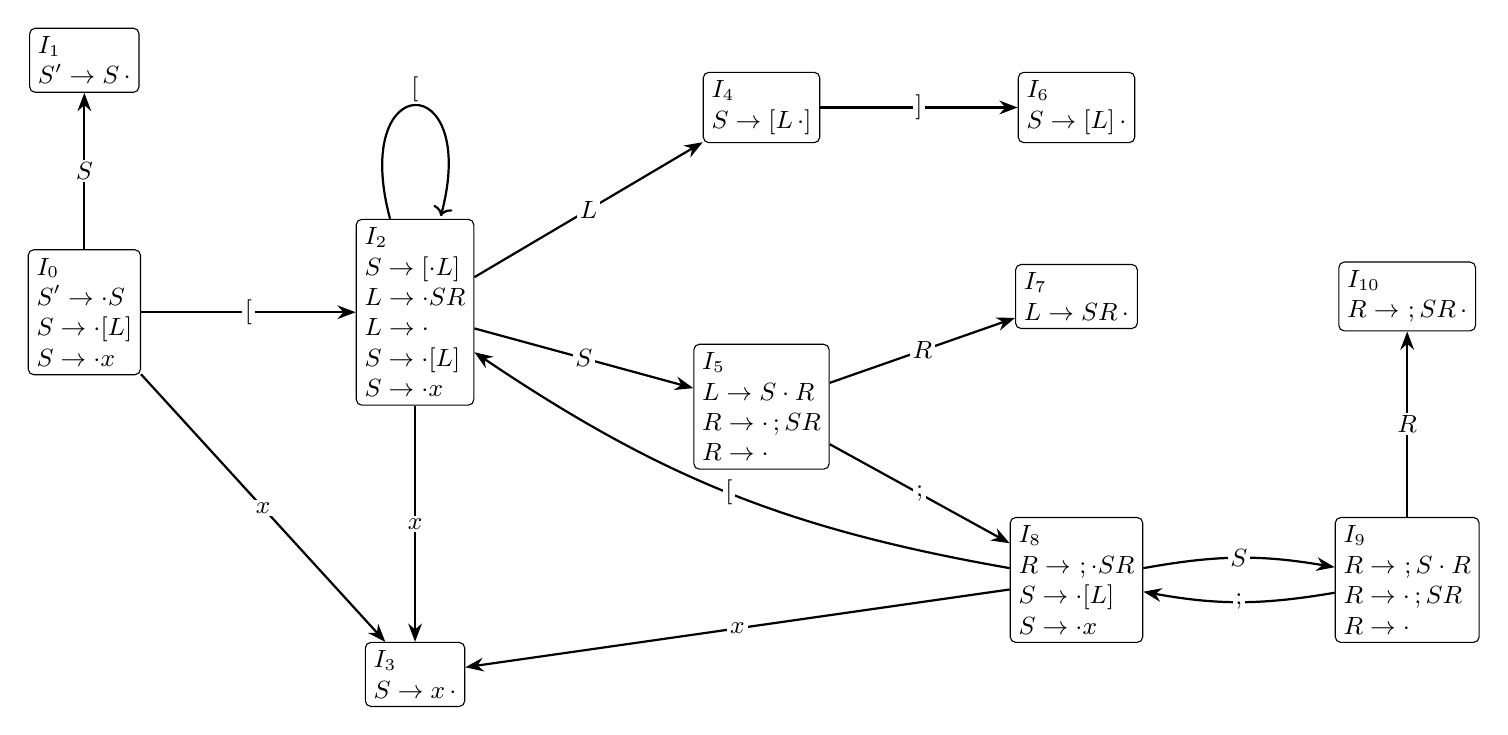
\begin{tikzpicture}[
  state/.style={draw, rounded corners=2pt, align=left, font=\small, inner sep=3pt},
  every edge/.style={draw, -{Stealth}, thick},
  lbl/.style={font=\small, fill=white, inner sep=1pt}]
  \node[state] (I0) at (0,0)    {$I_0$\\ $S' \to \cdot S$\\ $S \to \cdot [L]$\\ $S \to \cdot x$};
  \node[state] (I1) at (0,3.2)  {$I_1$\\ $S' \to S\,\cdot$};
  \node[state] (I2) at (4.2,0)  {$I_2$\\ $S \to [\cdot L]$\\ $L \to \cdot SR$\\ $L \to \cdot$\\ $S \to \cdot [L]$\\ $S \to \cdot x$};
  \node[state] (I3) at (4.2,-4.6) {$I_3$\\ $S \to x\,\cdot$};
  \node[state] (I4) at (8.6,2.6) {$I_4$\\ $S \to [L\,\cdot]$};
  \node[state] (I6) at (12.6,2.6) {$I_6$\\ $S \to [L]\,\cdot$};
  \node[state] (I5) at (8.6,-1.2) {$I_5$\\ $L \to S\cdot R$\\ $R \to \cdot\, ;SR$\\ $R \to \cdot$};
  \node[state] (I7) at (12.6,0.2) {$I_7$\\ $L \to SR\,\cdot$};
  \node[state] (I8) at (12.6,-3.4) {$I_8$\\ $R \to\ ;\cdot SR$\\ $S \to \cdot [L]$\\ $S \to \cdot x$};
  \node[state] (I9) at (16.8,-3.4) {$I_9$\\ $R \to\ ;S\cdot R$\\ $R \to \cdot\, ;SR$\\ $R \to \cdot$};
  \node[state] (I10) at (16.8,0.2) {$I_{10}$\\ $R \to\ ;SR\,\cdot$};

  \path (I0) edge node[lbl] {$S$} (I1)
        (I0) edge node[lbl] {$[$} (I2)
        (I0) edge node[lbl] {$x$} (I3)
        (I2) edge[loop above] node[lbl] {$[$} (I2)
        (I2) edge node[lbl] {$L$} (I4)
        (I2) edge node[lbl] {$S$} (I5)
        (I2) edge node[lbl] {$x$} (I3)
        (I4) edge node[lbl] {$]$} (I6)
        (I5) edge node[lbl] {$R$} (I7)
        (I5) edge node[lbl] {$;$} (I8)
        (I8) edge[bend left=12] node[lbl] {$[$} (I2)
        (I8) edge node[lbl] {$x$} (I3)
        (I8) edge[bend left=10] node[lbl] {$S$} (I9)
        (I9) edge[bend left=10] node[lbl] {$;$} (I8)
        (I9) edge node[lbl] {$R$} (I10);
\end{tikzpicture}}
\caption{LR(0) automaton of the grammar (canonical collection of sets of LR(0) items).}
\label{fig:lr0}
\end{figure}

Algorithm~4.46 builds the table below; \code{si} means shift~$i$, \code{rj} means reduce by production~$j$, and
\code{acc} means accept. No entry received two actions, so the grammar is SLR(1). For example, in
$I_2$ the item $L \to \cdot$ produces a reduce by (4) only on $\Follow(L) = \{]\}$, and this does not clash with
the shifts on \code{[} and \code{x}.

\begin{table}[H]
\centering
\begin{tabular}{@{}c|ccccc|ccc@{}}
\toprule
 & \multicolumn{5}{c|}{\Action} & \multicolumn{3}{c}{\Goto} \\
State & \code{;} & \code{[} & \code{]} & \code{x} & \code{\$} & $L$ & $R$ & $S$ \\
\midrule
0 &    & s2 &    & s3 &     &   &    & 1 \\
1 &    &    &    &    & acc &   &    &   \\
2 &    & s2 & r4 & s3 &     & 4 &    & 5 \\
3 & r2 &    & r2 &    & r2  &   &    &   \\
4 &    &    & s6 &    &     &   &    &   \\
5 & s8 &    & r6 &    &     &   & 7  &   \\
6 & r1 &    & r1 &    & r1  &   &    &   \\
7 &    &    & r3 &    &     &   &    &   \\
8 &    & s2 &    & s3 &     &   &    & 9 \\
9 & s8 &    & r6 &    &     &   & 10 &   \\
10 &   &    & r5 &    &     &   &    &   \\
\bottomrule
\end{tabular}
\caption{SLR(1) parsing table (Algorithm 4.46), as printed by \code{python slr1.py}.}
\end{table}

Since the grammar is both LL(1) and SLR(1), \code{main.py} asks the user to choose a parser (case~1 of Section~2.2.2).

\subsection{One string parsed step by step}

Here is the string \code{[x;[]]} parsed with each parser. Figure~\ref{lst:ll} shows the moves of the LL(1) parser
(\code{python ll1.py < tests/report\_grammar.txt}). As in Fig.~4.21 of the book, each row shows the configuration after the action of that row, and the top of the stack is on the left.

\begin{figure}[H]
\begin{lstlisting}
MATCHED             STACK               INPUT               ACTION
                    S$                  [x;[]]$
                    [L]$                [x;[]]$             output S -> [L]
[                   L]$                 x;[]]$              match [
[                   SR]$                x;[]]$              output L -> SR
[                   xR]$                x;[]]$              output S -> x
[x                  R]$                 ;[]]$               match x
[x                  ;SR]$               ;[]]$               output R -> ;SR
[x;                 SR]$                []]$                match ;
[x;                 [L]R]$              []]$                output S -> [L]
[x;[                L]R]$               ]]$                 match [
[x;[                ]R]$                ]]$                 output L -> e
[x;[]               R]$                 ]$                  match ]
[x;[]               ]$                  ]$                  output R -> e
[x;[]]              $                   $                   match ]
yes
\end{lstlisting}
\caption{Moves of the predictive parser (Algorithm 4.34) on \code{[x;[]]}.}
\label{lst:ll}
\end{figure}

Figure~\ref{lst:lr} shows the moves of the LR parser (\code{python slr1.py < tests/report\_grammar.txt}). As in Fig.~4.38 of the book, each row shows the action that is applied to that configuration.

\begin{figure}[H]
\begin{lstlisting}
STACK                    SYMBOLS             INPUT               ACTION
0                                            [x;[]]$             shift 2
0 2                      [                   x;[]]$              shift 3
0 2 3                    [x                  ;[]]$               reduce by S -> x
0 2 5                    [S                  ;[]]$               shift 8
0 2 5 8                  [S;                 []]$                shift 2
0 2 5 8 2                [S;[                ]]$                 reduce by L -> e
0 2 5 8 2 4              [S;[L               ]]$                 shift 6
0 2 5 8 2 4 6            [S;[L]              ]$                  reduce by S -> [L]
0 2 5 8 9                [S;S                ]$                  reduce by R -> e
0 2 5 8 9 10             [S;SR               ]$                  reduce by R -> ;SR
0 2 5 7                  [SR                 ]$                  reduce by L -> SR
0 2 4                    [L                  ]$                  shift 6
0 2 4 6                  [L]                 $                   reduce by S -> [L]
0 1                      S                   $                   accept
yes
\end{lstlisting}
\caption{Moves of the LR parser (Algorithm 4.44) on \code{[x;[]]}.}
\label{lst:lr}
\end{figure}

\subsection{Tests of Items 1 and 2}

The three examples of the assignment produce exactly the expected output:
\begin{itemize}
  \item Example~1 gives \code{Grammar is SLR(1).} and then \code{yes yes no}.
  \item Example~2 shows the menu and gives \code{yes yes no}.
  \item Example~3 gives \code{Grammar is neither LL(1) nor SLR(1).}
\end{itemize}
We also tested the following cases (all files are in \code{tests/}):
\begin{itemize}
  \item A grammar that is LL(1) but not SLR(1): $S \to AaAb \mid BbBa$, $A \to \varepsilon$, $B \to \varepsilon$. In $I_0$ there is a reduce/reduce conflict between $A \to \cdot$ and $B \to \cdot$ on \code{a} and \code{b}.
  \item The empty string (line \code{e}) with $S \to aSb \mid \varepsilon$.
  \item A grammar whose first line is not the one of $S$.
  \item Strings with characters that are not terminals.
\end{itemize}
For the expression grammar of the book, the program prints the same LR(0) automaton (Fig.~4.31), the
same SLR table (Fig.~4.37) and the same moves (Fig.~4.38) as the book.

\section{Item 3: syntax-directed definition}

\subsection{Step 1: the grammar}

Our language is numbers written with a prefix that gives their base: \code{b} (binary), \code{o} (octal) or
\code{d} (decimal). Examples are \code{b101}, \code{o17} and \code{d2026}.
\begin{center}
\begin{tabular}{l}
\code{5}\\
\code{S -> BN}\\
\code{B -> b o d}\\
\code{N -> DR}\\
\code{R -> DR e}\\
\code{D -> 0 1 2 3 4 5 6 7 8 9}
\end{tabular}
\end{center}
The grammar meets the three conditions of the assignment:
\begin{itemize}
  \item \textbf{G1.} It follows the conventions of Section~2.2 and is both LL(1) and SLR(1) (\code{tests/sdd\_grammar.txt}). The strings are parsed with our LL(1) parser.
  \item \textbf{G2.} It has 5 nonterminals and 17 productions, and $R$ is recursive.
  \item \textbf{G3.} The book has SDDs for binary numbers (Exercises 5.2.4 and 5.2.5) and an inherited accumulator (Fig.~5.4). Ours is different in three ways: the base is not fixed but comes from a prefix and is passed down the tree as an inherited attribute; the SDD supports three bases; and each digit is checked against the base. A string such as \code{b102} is syntactically correct, but its value is \code{error}.
\end{itemize}

\subsection{Step 2: attributes and semantic rules}

\begin{table}[H]
\centering
\small
\begin{tabular}{@{}cllll@{}}
\toprule
Symbol & Attribute & Kind & Type & Meaning \\
\midrule
$S$ & \code{val} & synthesized & integer or \code{error} & value of the number \\
$B$ & \code{base} & synthesized & integer & base given by the prefix (2, 8 or 10) \\
$N$ & \code{base} & inherited & integer & base in which the digits are read \\
$N$ & \code{val} & synthesized & integer or \code{error} & value of the digits \\
$R$ & \code{base} & inherited & integer & base in which the digits are read \\
$R$ & \code{acc} & inherited & integer or \code{error} & value of the digits to the left of $R$ \\
$R$ & \code{val} & synthesized & integer or \code{error} & value of all the digits \\
$D$ & \code{val} & synthesized & integer & value of one digit \\
terminals & \code{lexval} & synthesized & character & the character itself (given by the ``scanner'') \\
\bottomrule
\end{tabular}
\caption{Attributes of the SDD.}
\end{table}

\begin{table}[H]
\centering
\begin{tabular}{@{}ll@{}}
\toprule
Production & Semantic rules \\
\midrule
$S \to B\,N$ & $N.base = B.base$ \\
             & $S.val = N.val$ \\[2pt]
$B \to b$ & $B.base = base\_of(b.lexval)$ \quad (the same rule for $B \to o$ and $B \to d$) \\[2pt]
$N \to D\,R$ & $R.base = N.base$ \\
             & $R.acc = first\_digit(D.val, N.base)$ \\
             & $N.val = R.val$ \\[2pt]
$R \to D\,R_1$ & $R_1.base = R.base$ \\
               & $R_1.acc = accumulate(R.acc, D.val, R.base)$ \\
               & $R.val = R_1.val$ \\[2pt]
$R \to \varepsilon$ & $R.val = R.acc$ \\[2pt]
$D \to k$ \ ($k = 0,\dots,9$) & $D.val = digit\_value(k.lexval)$ \\
\bottomrule
\end{tabular}
\caption{The SDD, in the format of Fig.~5.1.}
\end{table}

\noindent The semantic functions are:
\begin{itemize}
  \item $base\_of(\code{b}) = 2$, $base\_of(\code{o}) = 8$ and $base\_of(\code{d}) = 10$;
  \item $digit\_value(k)$ is the integer value of the digit~$k$;
  \item $accumulate(acc, d, base) = acc \cdot base + d$, or \code{error} if $acc = \code{error}$ or $d \ge base$;
  \item $first\_digit(d, base) = accumulate(0, d, base)$.
\end{itemize}

\noindent We checked the two conditions of Section~5.1.1 for every production:
\begin{itemize}
  \item Each rule defines either a synthesized attribute of the head ($S.val$, $B.base$, $N.val$, $R.val$, $D.val$) or an inherited attribute of a body symbol ($N.base$, $R.base$, $R.acc$, $R_1.base$, $R_1.acc$). It uses only attributes of the symbols of that same production.
  \item In every production, each synthesized attribute of the head and each inherited attribute of the body nonterminals is defined exactly once.
\end{itemize}
The start symbol $S$ has no inherited attributes.

\subsection{Step 3: example by hand}

We use the string \code{b101} (four terminals), whose value is $1\cdot 4 + 0\cdot 2 + 1 = 5$.

\todo{Insert here the parse tree of \code{b101} annotated with all its attribute values, the dependency
graph (one vertex per attribute of each node, and one edge from each used attribute to the defined
attribute), and one valid topological order. Do them by hand (drawn or scanned, or transcribed to TikZ),
as the assignment requires. Then compare them with the output of the program below.}

\medskip
\noindent Output of \code{python sdd.py} for \code{b101}. The number in brackets identifies each node:
\begin{lstlisting}
Annotated parse tree:
S[1]  val=5
    B[2]  base=2
        b[3]  lexval=b
    N[4]  base=2, val=5
        D[5]  val=1
            1[6]  lexval=1
        R[7]  base=2, acc=1, val=5
            D[8]  val=0
                0[9]  lexval=0
            R[10]  base=2, acc=2, val=5
                D[11]  val=1
                    1[12]  lexval=1
                R[13]  base=2, acc=5, val=5
                    e
Evaluation order:
    1. b[3].lexval        8. D[11].val         15. R[13].acc
    2. 1[6].lexval        9. N[4].base         16. R[13].val
    3. 0[9].lexval       10. R[7].base         17. R[10].val
    4. 1[12].lexval      11. R[7].acc          18. R[7].val
    5. B[2].base         12. R[10].base        19. N[4].val
    6. D[5].val          13. R[10].acc         20. S[1].val
    7. D[8].val          14. R[13].base
S.val = 5
\end{lstlisting}
(To save space, the evaluation order is shown here in three columns; the program prints one attribute per line.)
\code{python sdd.py --step} also prints the 21 edges of the dependency graph, for example
\code{b[3].lexval -> B[2].base}, \code{B[2].base -> N[4].base}, \code{N[4].base -> R[7].acc},
\code{D[5].val -> R[7].acc} and \code{R[13].acc -> R[13].val}.

\subsection{Step 4: classification}

\begin{itemize}
  \item \textbf{It is not S-attributed} (Section~5.2.3), because it has inherited attributes ($N.base$, $R.base$, $R.acc$).
  \item \textbf{It is L-attributed} (Section~5.2.4). Every attribute is either synthesized or inherited, and every inherited attribute uses only inherited attributes of the head or attributes of symbols to its left:
  \begin{itemize}
    \item $N.base = B.base$ uses $B$, which is to the left of $N$ in $S \to BN$ (rule~2b).
    \item $R.base = N.base$ uses an inherited attribute of the head (rule~2a).
    \item $R.acc = first\_digit(D.val, N.base)$ uses $D$, which is to the left of $R$ (rule~2b), and an inherited attribute of the head (rule~2a).
    \item $R_1.base = R.base$ and $R_1.acc = accumulate(R.acc, D.val, R.base)$ use inherited attributes of the head $R$ (rule~2a) and $D$, which is to the left of $R_1$ (rule~2b).
  \end{itemize}
\end{itemize}
So the SDD is L-attributed, but not S-attributed. Even so, the evaluator does not use this property: it uses the general method of the dependency graph.

\subsection{Step 5: implementation}

\begin{enumerate}
  \item \textbf{SDD as data.} \code{sdd\_rules.py} contains only the grammar (as lines in the format of
  Section~2.2), the semantic functions and the dictionary \code{RULES}. For each production,
  \code{RULES} holds the list of its rules. A rule is a tuple
  \code{(defined attribute, used attributes, function)}, and an attribute is a pair
  \code{(position, name)}: position~0 is the head and positions $1,\dots,n$ are the body symbols. For example, the rule
  $R_1.acc = accumulate(R.acc, D.val, R.base)$ of $R \to DR_1$ is written
  \code{((2,"acc"), [(0,"acc"), (1,"val"), (0,"base")], accumulate)}. The evaluator \code{sdd.py} does not know
  anything about this SDD.
  \item \textbf{Parse tree.} The string is parsed with the LL(1) parser of Item~2. Its stack holds parse-tree nodes, not only symbols. When $X$ is replaced by $Y_1 \cdots Y_k$, the nodes of the $Y_i$ become the children of the node of~$X$; the book mentions this possibility after Fig.~4.20. Each node stores its symbol, its production, its children and its attribute values.
  \item \textbf{Dependency graph} (\code{build\_graph}, Section~5.2.1). For each internal node, the program takes the rules of its production. For each rule, it adds an edge from each attribute that the rule uses to the attribute that it defines. The leaves provide their \code{lexval}.
  \item \textbf{Order and evaluation} (\code{topological\_order} and \code{evaluate}, Section~5.2.2). As the book explains, the program repeatedly takes a vertex with no incoming edges, appends it to the order and removes it. To ``remove'' it, it keeps a count of incoming edges for each vertex. If at some point vertices remain but none has zero incoming edges, the graph has a cycle: the program prints that the SDD is circular and stops. Otherwise, it evaluates the attributes in that order, calling the function of each rule with the values of the attributes it uses.
  \item \textbf{Output.} For each string, the program prints \code{no} if the string is not in the language. Otherwise, it prints the annotated parse tree, the evaluation order and the value of $S.val$.
\end{enumerate}
With \code{--step}, the program works as a text visualizer. It prints the edges of the graph and then evaluates one attribute each time the user presses Enter, showing the tree with the values known so far.

\subsection{Step 6: tests}

\begin{table}[H]
\centering
\begin{tabular}{@{}lll@{}}
\toprule
String & Case & Output \\
\midrule
\code{b0}   & shortest string of the language (2 terminals) & \code{S.val = 0} \\
\code{b101} & example of Step 3 & \code{S.val = 5} \\
\code{o17}  & octal & \code{S.val = 15} \\
\code{d2026} & decimal & \code{S.val = 2026} \\
\code{b102} & digit not valid in base 2 & \code{S.val = error} \\
\code{101}  & not in the language (no prefix) & \code{no} \\
\code{b}    & not in the language (no digits) & \code{no} \\
\code{e}    & empty string, not in the language & \code{no} \\
\code{b1111111111111111} & deep recursion (16 nested $R$, 85 attributes) & \code{S.val = 65535} \\
\bottomrule
\end{tabular}
\caption{Tests of the evaluator (\code{python sdd.py < tests/sdd\_strings.txt}).}
\end{table}

\paragraph{Circular SDD.} To show that the evaluator detects circular definitions, we temporarily changed the
rule $R.acc = first\_digit(D.val, N.base)$ of $N \to DR$ to $R.acc = R.val$. In the tree of any string,
$R.val$ depends on the $acc$ of the last $R$, which depends on the previous $acc$ values, and these in turn depend on $R.acc$. This
produces a cycle. The program's output is:
\begin{lstlisting}
Error: the SDD is circular (the dependency graph has a cycle).
\end{lstlisting}

\section{Problems found and how we solved them}

\begin{enumerate}
  \item \textbf{Repeated vertices in the dependency graph.} In our first version, when the program reached a leaf it created the vertex for its \code{lexval}. But that vertex sometimes already existed, because a rule of the parent node (for example $B.base = base\_of(b.lexval)$) had used it. Creating it again lost the edge from the parent rule and duplicated the vertex. As a result, \code{B.base} appeared before \code{b.lexval} in the evaluation order. We fixed it by creating each vertex only if it does not exist yet.
  \item \textbf{End of the LL(1) parse.} The loop of Fig.~4.20 stops when \$ is on top of the stack, but at that point part of the input may still be unread. For example, with $S \to a$ and the string \code{aa}, the stack becomes empty while one \code{a} is still unread. After the loop, we check that the current input symbol is \$.
  \item \textbf{Characters that are not terminals.} A string can contain characters that are not terminals of the grammar, such as an upper-case letter or \$. These strings are not in the language. However, a \$ in the middle of the string could make the LR parser accept before reading the whole string. The program therefore answers \code{no} for such strings without parsing them.
  \item \textbf{End of the input in the parser menu.} If the input ends without a \code{Q}, reading the menu letter used to give an empty line forever. Now \code{read\_line} returns \code{None} at the end of the input, and the menu treats it as \code{Q}.
  \item \textbf{LL(1) condition versus table conflicts.} We implemented the condition of Section~4.4.3, as the assignment requires. We also checked that it agrees with the absence of multiply-defined entries in the table built by Algorithm~4.31. The only case where they differ is a nonterminal that cannot be reached from $S$ and has two $\varepsilon$-alternatives: its \Follow{} set is empty, so its table row has no conflict. However, the condition (and therefore our program) still says that the grammar is not LL(1).
  \item \textbf{Numbering of the LR(0) states.} To compare our automaton with Fig.~4.31, the program tries the symbols $X$ that appear after a dot, in the order of the items. With this order, the states come out numbered as in the book.
\end{enumerate}

\section{Use of generative AI}

As stated in \code{README.md}, we used Claude Code (Anthropic, model Claude Opus 5.5) as a programming
assistant. This is what it did.

\begin{enumerate}
  \item \textbf{Implementation and debugging of the modules.}
  \begin{itemize}
    \item It read the assignment and proposed a work plan: the list of deliverables, the files of the program and the book section that each function had to follow. We asked for simple code that uses only the standard library and cites the book in each function, so that every member can explain it. The plan was adjusted to these requests before any code was written.
    \item It found and fixed the problems described in Section~5: the repeated \code{lexval} vertices, the end of the LL(1) parse, the characters that are not terminals and the end of the input in the menu.
    \item It wrote the input files of \code{tests/} and ran them. As an extra check that is not part of the submission, it compared the answers of both parsers with an exact membership test on 3\,086 random grammars and 455\,099 strings. In the same check it compared \code{is\_ll1} with the conflicts of the LL(1) table.
  \end{itemize}

  \item \textbf{Comparison with the book.}
  \begin{itemize}
    \item It extracted the text of Sections 4.4.2--4.4.4, 4.6.2--4.6.4 and 5.2.1--5.2.4. With it, it checked that each function follows the corresponding algorithm or figure step by step, and that the numbers cited in the code and in this report are correct.
    \item Following the book, it changed the format of the step-by-step output. In the LL(1) trace, each row shows the configuration after the action (Fig.~4.21). In the LR trace, each row shows the action applied to that configuration (Fig.~4.38).
    \item It checked that, for the expression grammar of the book, the program prints the same LR(0) automaton (Fig.~4.31), the same SLR table (Fig.~4.37) and the same moves (Fig.~4.38). It also changed the order in which the states are created so that they are numbered as in the book.
    \item It read Exercises 5.2.4 and 5.2.5 and Fig.~5.4 to compare our SDD with the ones in the book (condition G3).
  \end{itemize}
\end{enumerate}

\end{document}
